\documentclass{article}
\usepackage{algorithm2e}
\usepackage{graphicx}

\DeclareGraphicsExtensions{.png}

\title{Neural Networks: Assignment 1}
\author{Candidate Number: 18512}

\begin{document}
\maketitle

\begin{centering}
\subsubsection*{Abstract}
\end{centering}
\noindent This report will detail the implementation of a single layer perceptron for the purposes of binary classification and linear regression. \\
\indent The perceptron was implemented in Python. No Neural Network libraries or toolkits were used. Matplotlib and Numpy were used to produce graphs.
\vspace{4mm}

\section*{Part A: Classification}
\subsubsection*{Training Procedure}
In this part, sequential gradient descent was used, as it is somewhat simpler to implement, and for such simple cases, there is no benefit in terms of what we want to demonstrate, to using a more complicated implementation. Batch gradient descent will be used in part 2 of this assignment, however. \\
\indent The Perceptron Criterion error function is used, because unlike more naive error functions, Perceptron Criterion function yields a value proportional to the (sum of the) distance from the decision boundary. This is useful because any change in weights will correspond to a change in the value that the error function yields, which allows us to calculate the gradient of the error function, which in turn allows us to learn the optimum decision boundary via gradient descent. If a change in weights does not correspond to a change in error, we cannot determine whether the weight adjustment improved or worsened our learned function. \\
\indent The choice of learning rate for this part is not terribly important - it should be large enough that it does not cause the algorithm to do unnecessary extra iterations, and not be so great as to prevent convergence. 0.1 was found to be sufficient. \\

The training procedure for sequential gradient descent is as follows: \\

\begin{algorithm}[H]{\textbf{Procedure}: GradientDescentSequential} \\
    \KwIn{trainingData, weights, learningRate}
    \SetAlgoLined
    \Begin{
        \While{any element of trainingData is incorrectly classified} {
            \For{each instance in trainingData} {
                \If{instance is correctly classified} {
                    update weights in proportion to learningRate so instance is (closer to being) correctly classified
                }
            }
        }
    }
    \KwResult{weights}
\end{algorithm}
\vspace{4mm}

\noindent At the heart of this algorithm is the weight update step. To determine how we will update the weights, we use the Perceptron Criterion error function:
\[E^{Perc} = -\sum_{i = 1}^{m} \underline{x}_{i} . \underline{y}_{i} t_{i} \hspace{2mm} \textrm{for all misclassified} \hspace{2mm} x_{i}\]
With batch gradient descent, we can simply update every weight by the amount returned by this error function, multiplied by the learning rate. However, when applying this error function to sequential gradient descent, we get the following update rule:
\[w_{t+1} = w_{t} + \eta \underline{x}_{i} t_{i}\]
which is applied once for each instance over each epoch.
\subsection*{Question 1}
\indent For this question, initial weights were all zero as specified in the assignment brief.

\subsubsection*{Learnable Patterns}
The implemented single layer perceptron was able to learn four of the six given patterns:
\begin{center}
    \begin{tabular}{ l | c c c | l | c c c }
                & X1 & X2 & Label &         & X1 & X2 & Label \\
        \hline
        Pattern & 1  & 1  & +     & Pattern & 1  & 1  & -     \\
        Set 1   & 1  & 0  & -     & Set 2   & 1  & 0  & +     \\
                & 0  & 1  & +     &         & 0  & 1  & -     \\
                & 0  & 0  & -     &         & 0  & 0  & +     \\
        \hline
        Pattern & 1  & 1  & +     & Pattern & 1  & 1  & -     \\
        Set 3   & 1  & 0  & +     & Set 4   & 1  & 0  & -     \\
                & 0  & 1  & -     &         & 0  & 1  & +     \\
                & 0  & 0  & -     &         & 0  & 0  & +     \\
    \end{tabular}
\end{center}
Pattern sets 1 \& 2 are equivalent modulo the choice of class names, and as a result are learnt in the same number of iterations (2). The same is the case for pattern sets 3 \& 4. The ones that cannot be learnt are just so because they are not linearly separable i.e. there exists no linear boundary that separates all instances of one class from all instances of the other. These are given below:
\begin{center}
    \begin{tabular}{ l | c c c | l | c c c }
                & X1 & X2 & Label &         & X1 & X2 & Label \\
        \hline
        Pattern & 1  & 1  & +     & Pattern & 1  & 1  & -     \\
        Set 5   & 1  & 0  & -     & Set 6   & 1  & 0  & +     \\
                & 0  & 1  & -     &         & 0  & 1  & +     \\
                & 0  & 0  & +     &         & 0  & 0  & -     \\
    \end{tabular}
\end{center}
The following table shows the learned weights and number of iterations for each set of learnable patterns:
\begin{center}
    \begin{tabular}{ c | c | c | c | c }
        Pattern Set & Bias & Weight 1 & Weight 2 & Iterations \\
        \hline
        1           & 0    & -0.2     & 0        & 2          \\
        \hline
        2           & -0.1 & 0.2      & 0        & 2          \\
        \hline
        3           & 0    & 0        & -0.1     & 2          \\
        \hline
        4           & -0.1 & 0        & 0.1      & 2          \\
    \end{tabular}
\end{center}

The graphs below show the state of the decision boundary after each iteration, for pattern set 4: \\

\centerline{\textbf{Initial State}: Bias = 0, W1 = 0, W2 = 0}
\centerline{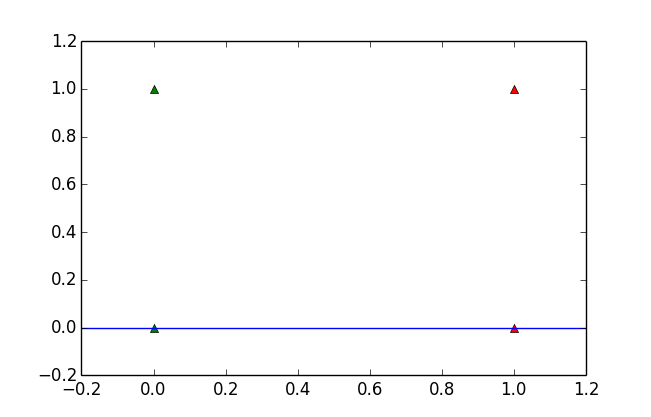
\includegraphics[width=200px]{partA1_iter1}}
\vspace{6mm}
\centerline{\textbf{After First Iteration}: Bias = 0, W1 = 0, W2 = 0.1}
\centerline{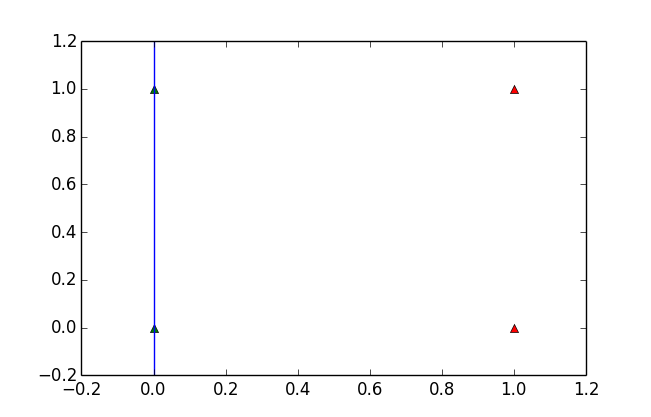
\includegraphics[width=200px]{partA1_iter2}}
\vspace{6mm}
\centerline{\textbf{After Second Iteration} (final state): Bias = -0.1, W1 = 0, W2 = 0.1}
\centerline{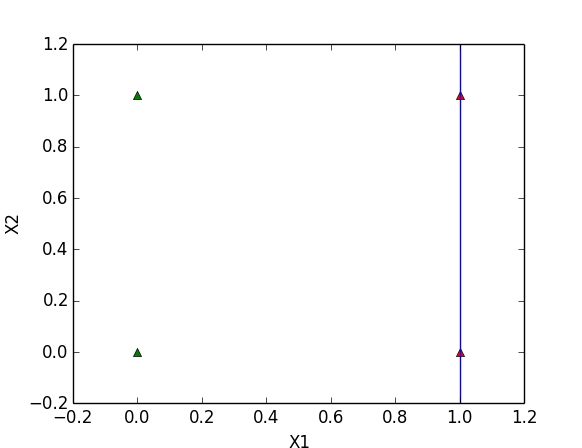
\includegraphics[width=200px]{partA1_iter3}}

\subsection*{Question 2}
In this question, the same code was used to learn the decision boundary as with question 1. The graph below shows the output of an example run of the implementation for this question: \\\\
\centerline{\textbf{Example Instances \& Decision Boundary}}
\centerline{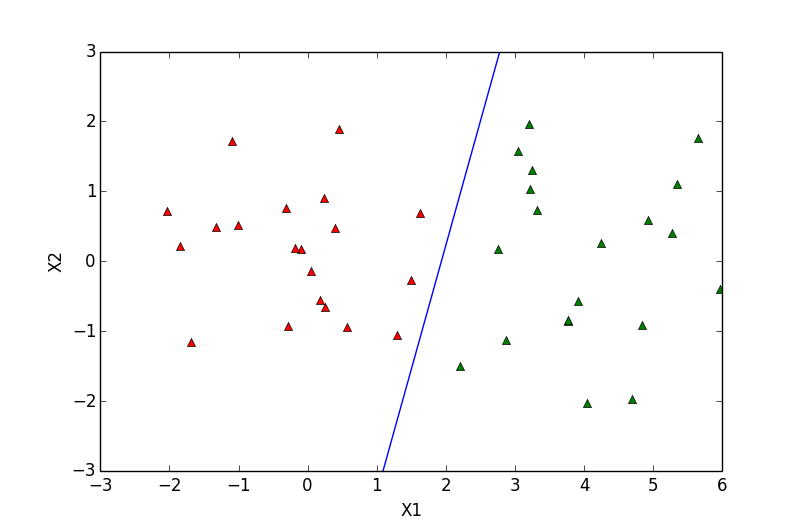
\includegraphics[width=400px]{partA2_1}}

\noindent The graph below shows the boundary learned for a non-linearly separable set of points - the decision boundary is not able to classify all points correctly, and, moreover, it is far from optimal, as we can see from the graph. It does not describe the data well. Since the algorithm used does not terminate for non-linearly separable data (it will never be the case that all points are correctly classified), an iteration limit must be imposed for non-linearly separable data. In the example below, the algorithm was limited to 100 iterations (over all data points i.e. 100 epochs). \\\\
\centerline{\textbf{Example of non-linearly separable Instances \& resulting Decision Boundary}}
\centerline{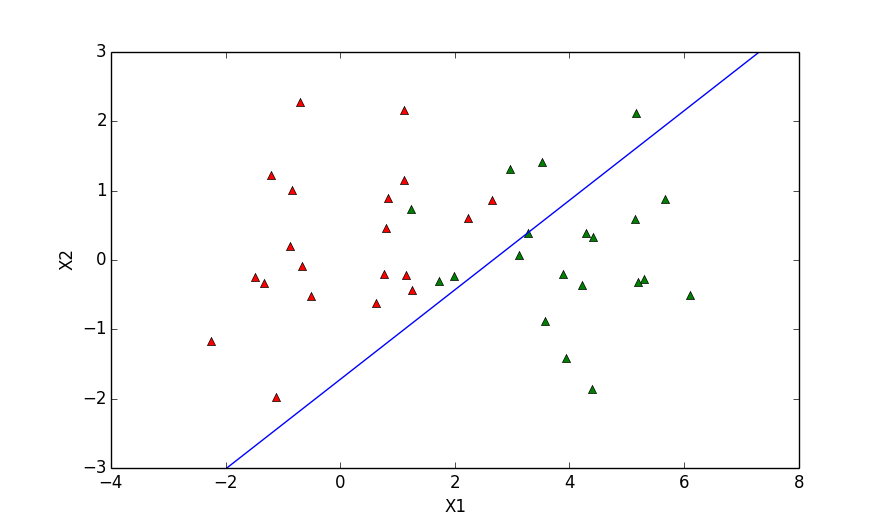
\includegraphics[width=400px]{partA2_2}}
\vspace{6mm}

\noindent The graphs below show how the decision boundary moves after each iteration for a set of points that were learned in 3 iterations: \\
\begin{center}
\textbf{Initial State}: Bias = 0, W1 = 0, W2 = 0 \\
\centerline{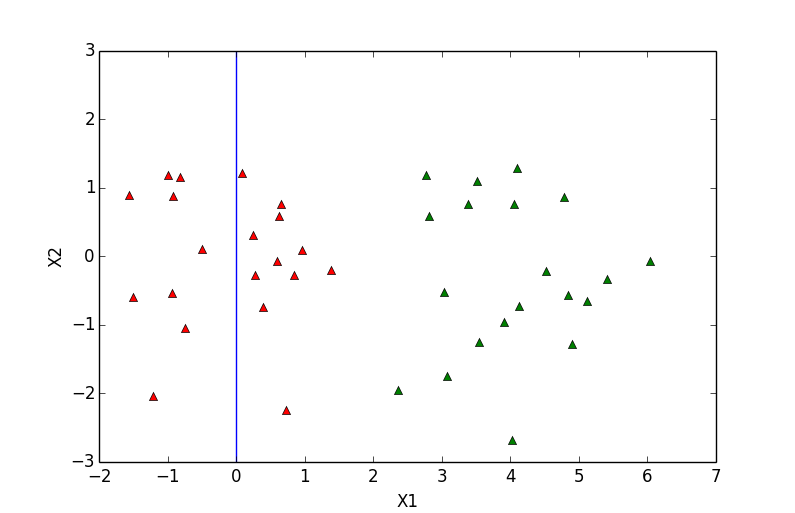
\includegraphics[width=400px, height=220px]{partA2_iter0}}
\vspace{2mm}
\rule{8cm}{0.4pt} \\
\vspace{2mm}
\textbf{After First Iteration}: Bias = 0.3, W1 = -0.22, W2 = 0.04 \\
\centerline{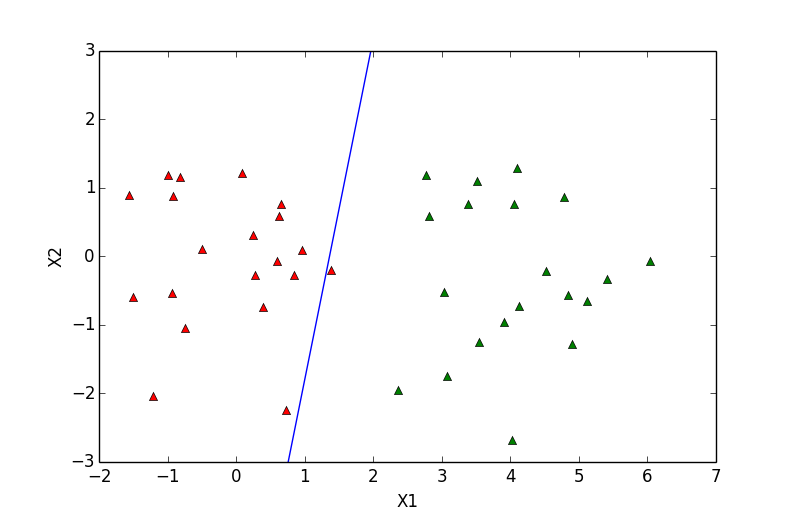
\includegraphics[width=400px, height=220px]{partA2_iter1}}
\vspace{2mm}
\rule{8cm}{0.4pt} \\
\vspace{2mm}
\textbf{After Second Iteration}: Bias = 0.4, W1 = -0.43, W2 = -0.05 \\
\centerline{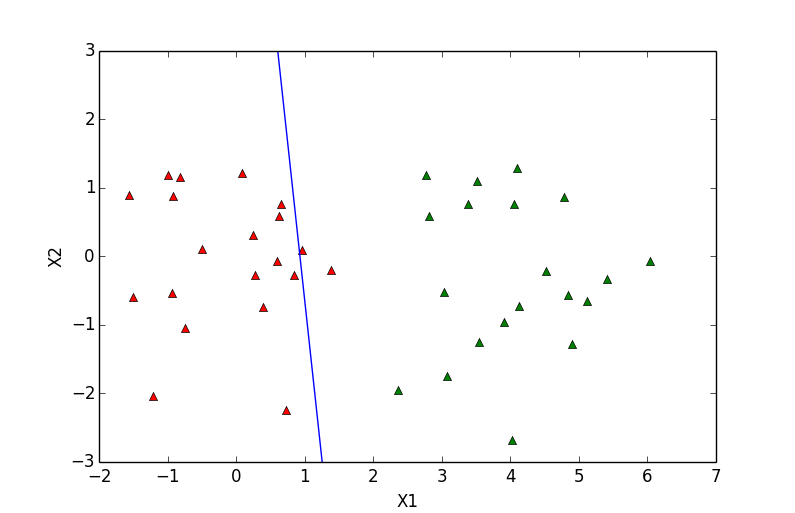
\includegraphics[width=400px, height=220px]{partA2_iter2}}
\vspace{2mm}
\rule{8cm}{0.4pt} \\
\vspace{2mm}
\textbf{After Third Iteration} (final state): Bias = 0.5, W1 = -0.33, W2 = -0.04 \\
\centerline{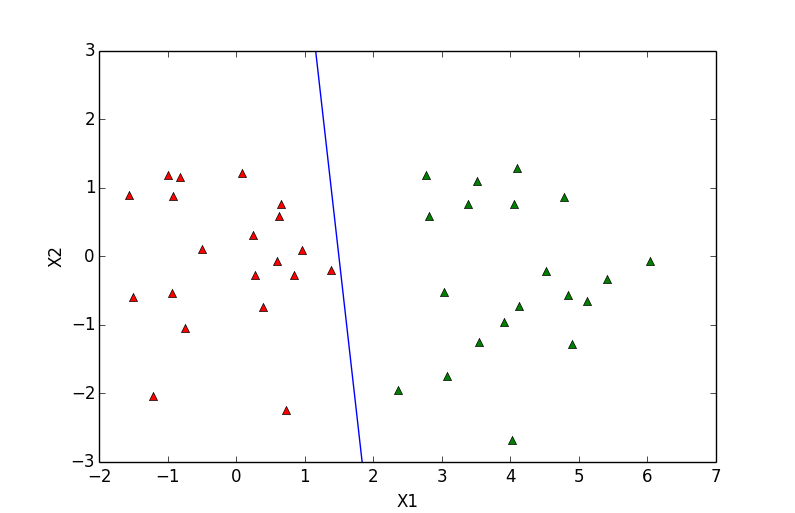
\includegraphics[width=400px, height=220px]{partA2_iter3}}
\vspace{2mm}
\rule{8cm}{0.4pt} \\
\vspace{2mm}
\end{center}

\noindent Given the function used to generate the data, the ideal decision boundary would be the vertical line X1 = 2. In all cases we have seen, the noise in the data prevents such a line from being learned. With a larger dataset, this noise would likely not affect the line to such a degree, however the larger the dataset becomes, the less likely it is that the dataset is linearly separable.

\textbf{TODO tanh activation function}
\section*{Part B: Regression}
\subsection*{Question 1}

\subsection*{Question 2}

\end{document}
